% 2017-01-27 - Bruno Iran Ferreira Maciel - bifm@cin.ufpe.br
\documentclass[xcolor=table,smaller,aspectratio=169]{beamer}

% ----------------------------------------------------------
% Customização p/ o estilo bifm
% ----------------------------------------------------------
\usepackage{bifm}
% ----------------------------------------------------------
% Configura parâmetros p/ o estilo bifm
% ----------------------------------------------------------



\makeatletter%
\@ifclassloaded{beamer}%
{
%----------------------------------------------------------
% glossário e acrônimos
%
\usepackage[acronym]{glossaries} %GLOSSÁRIO
%\GlsSetXdyCodePage{utf8}
\glsnoexpandfields
\glsaddall
\makeglossaries
\newglossarystyle{dotglos}{%
	\setglossarystyle{list}%
	\renewcommand*{\glossentry}[2]{%
		\item[\glsentryitem{##1}\glstarget{##1}{\glossentryname{##1}}]
		\ifglshassymbol{##1}{[\glossentrysymbol{##1}]\quad}{}%
		\emph{\glossentrydesc{##1}}%
		\unskip\leaders\hbox to 2.9mm{\hss.}\hfill##2}%
	\renewcommand*{\glsgroupskip}{}%
}
% \newglossarystyle{dotglos}{%
% 	\setglossarystyle{list}% base this style on the list style
% 	\renewcommand*{\glossentry}[2]{%
% 		\item[\glsentryitem{##1}%
% 		\glstarget{##1}{\glossentryname{##1}}]
% 		\glossentrydesc{##1}\glspostdescription\space
% 		\unskip\leaders\hbox to 2.9mm{\hss.}\hfill\ifnum\glsentryprevcount{##1}>1 pp.\else p.\fi\ ##2}%
% }
\setglossarystyle{dotglos}
%----------------------------------------------------------
	}%
{}%
\makeatother%


%----------------------------------------------------------
% alinhar texto justificado
%
\usepackage{ragged2e}
%----------------------------------------------------------



\newcommand\sbullet[1][.5]{\mathbin{\ThisStyle{\vcenter{\hbox{%
					\scalebox{#1}{$\SavedStyle\bullet$}}}}}%
}


% para codigos


\usepackage{listings}
\usepackage{listingsutf8}
\usepackage{inconsolata}

\definecolor{dkgreen}{rgb}{0,0.6,0}
\definecolor{gray}{rgb}{0.5,0.5,0.5}
\definecolor{mauve}{rgb}{0.58,0,0.82}

\lstdefinestyle{CBruno}{
  inputencoding=utf8,
%   extendedchars=false,
    language=java,
    backgroundcolor=\color{white},
    commentstyle=\color{dkgreen},
    % keywordstyle=\color{blue},
    % keywordstyle={[2]\color{magenta}},
    numberstyle=\tiny\color{gray},
    stringstyle=\color{mauve},
    % basicstyle=\footnotesize,
    basicstyle=\tiny,
    comment=[l]{\#},
    escapechar=@,
    escapeinside={\%*}{\text{\%}*)},
    % escapeinside={;@}{\^^M},
    otherkeywords={*,...},
    % escapeinside={\%*}{*)},
    % keywords={@relation,@attribute,@data},
    % morekeywords=[2]{real,integer,numeric,string,date},
    breakatwhitespace=true,
    breaklines=true,
    captionpos=b,
    keepspaces=true,
    firstnumber=1,
    numbers=left,
    numbersep=5pt,
    showspaces=false,
    showstringspaces=false,
    showtabs=false,
    tabsize=2,
    frame=single,
    rulecolor=\color{black},
    keywordstyle=\color{blue},
    % morekeywords={*,...},
    % alsoletter={., [\_]},
    texcl=true,
    alsoletter ={_},
    otherkeywords = {!,!=,~,$,*,\&,\%/\%,\%*\%,\%\%,<-,<<-},
    % morecomment=[s][\color{black}]{<!--}{-->},
    stepnumber=1,
    % morecomment=[l][]{//}, 
    % morecomment=[s][]{/*}{*/},
    % morestring=[b]",
    % morestring=[b]',
    extendedchars=true,
    literate=*
    {á}{{\'a}}1 {é}{{\'e}}1 {í}{{\'i}}1 {ó}{{\'o}}1 {ú}{{\'u}}1
    {Á}{{\'A}}1 {É}{{\'E}}1 {Í}{{\'I}}1 {Ó}{{\'O}}1 {Ú}{{\'U}}1
    {à}{{\`a}}1 {è}{{\`e}}1 {ì}{{\`i}}1 {ò}{{\`o}}1 {ù}{{\`u}}1
    {À}{{\`A}}1 {È}{{\'E}}1 {Ì}{{\`I}}1 {Ò}{{\`O}}1 {Ù}{{\`U}}1
    {ä}{{\"a}}1 {ë}{{\"e}}1 {ï}{{\"i}}1 {ö}{{\"o}}1 {ü}{{\"u}}1
    {Ä}{{\"A}}1 {Ë}{{\"E}}1 {Ï}{{\"I}}1 {Ö}{{\"O}}1 {Ü}{{\"U}}1
    {â}{{\^a}}1 {ê}{{\^e}}1 {î}{{\^i}}1 {ô}{{\^o}}1 {û}{{\^u}}1
    {ã}{{\~a}}1 {ẽ}{{\~e}}1 {ĩ}{{\~i}}1 {õ}{{\~o}}1 {ũ}{{\~u}}1
    {Â}{{\^A}}1 {Ê}{{\^E}}1 {Î}{{\^I}}1 {Ô}{{\^O}}1 {Û}{{\^U}}1
    {œ}{{\oe}}1 {Œ}{{\OE}}1 {æ}{{\ae}}1 {Æ}{{\AE}}1 {ß}{{\ss}}1
    {ç}{{\c c}}1 {Ç}{{\c C}}1 {ø}{{\o}}1 {å}{{\r a}}1 {Å}{{\r A}}1
    {€}{{\EUR}}1 {£}{{\pounds}}1 {^}{\text{\^{}}}1 {\\}{{$\textbackslash$}}1
    {\%}{{\%}}1 
}

\lstdefinestyle{javaBruno}{
  inputencoding=utf8,
%   extendedchars=false,
    language=java,
    backgroundcolor=\color{white},
    commentstyle=\color{dkgreen},
    % keywordstyle=\color{blue},
    % keywordstyle={[2]\color{magenta}},
    numberstyle=\tiny\color{gray},
    stringstyle=\color{mauve},
    % basicstyle=\footnotesize,
    basicstyle=\tiny,
    comment=[l]{\#},
    escapechar=@,
    escapeinside={\%*}{\text{\%}*)},
    % escapeinside={;@}{\^^M},
    otherkeywords={*,...},
    % escapeinside={\%*}{*)},
    % keywords={@relation,@attribute,@data},
    % morekeywords=[2]{real,integer,numeric,string,date},
    breakatwhitespace=true,
    breaklines=true,
    captionpos=b,
    keepspaces=true,
    firstnumber=1,
    numbers=left,
    numbersep=5pt,
    showspaces=false,
    showstringspaces=false,
    showtabs=false,
    tabsize=2,
    frame=single,
    rulecolor=\color{black},
    keywordstyle=\color{blue},
    % morekeywords={*,...},
    % alsoletter={., [\_]},
    texcl=true,
    alsoletter ={_},
    otherkeywords = {!,!=,~,$,*,\&,\%/\%,\%*\%,\%\%,<-,<<-},
    % morecomment=[s][\color{black}]{<!--}{-->},
    stepnumber=1,
    % morecomment=[l][]{//}, 
    % morecomment=[s][]{/*}{*/},
    % morestring=[b]",
    % morestring=[b]',
    extendedchars=true,
    literate=*
    {á}{{\'a}}1 {é}{{\'e}}1 {í}{{\'i}}1 {ó}{{\'o}}1 {ú}{{\'u}}1
    {Á}{{\'A}}1 {É}{{\'E}}1 {Í}{{\'I}}1 {Ó}{{\'O}}1 {Ú}{{\'U}}1
    {à}{{\`a}}1 {è}{{\`e}}1 {ì}{{\`i}}1 {ò}{{\`o}}1 {ù}{{\`u}}1
    {À}{{\`A}}1 {È}{{\'E}}1 {Ì}{{\`I}}1 {Ò}{{\`O}}1 {Ù}{{\`U}}1
    {ä}{{\"a}}1 {ë}{{\"e}}1 {ï}{{\"i}}1 {ö}{{\"o}}1 {ü}{{\"u}}1
    {Ä}{{\"A}}1 {Ë}{{\"E}}1 {Ï}{{\"I}}1 {Ö}{{\"O}}1 {Ü}{{\"U}}1
    {â}{{\^a}}1 {ê}{{\^e}}1 {î}{{\^i}}1 {ô}{{\^o}}1 {û}{{\^u}}1
    {ã}{{\~a}}1 {ẽ}{{\~e}}1 {ĩ}{{\~i}}1 {õ}{{\~o}}1 {ũ}{{\~u}}1
    {Â}{{\^A}}1 {Ê}{{\^E}}1 {Î}{{\^I}}1 {Ô}{{\^O}}1 {Û}{{\^U}}1
    {œ}{{\oe}}1 {Œ}{{\OE}}1 {æ}{{\ae}}1 {Æ}{{\AE}}1 {ß}{{\ss}}1
    {ç}{{\c c}}1 {Ç}{{\c C}}1 {ø}{{\o}}1 {å}{{\r a}}1 {Å}{{\r A}}1
    {€}{{\EUR}}1 {£}{{\pounds}}1 {^}{\text{\^{}}}1 {\\}{{$\textbackslash$}}1
    {\%}{{\%}}1 
}

\lstset{style=javaBruno}




\definecolor{cinColor}{HTML}{008f4c} %cor padrão

\definecolor{consulta}{HTML}{f0f0f5} %cor padrão
\definecolor{consultatitulo}{HTML}{9595b7} %cor padrão

\makeatletter%
\@ifclassloaded{beamer}%
  {\setbeamercolor{saibamais}{fg=cinzaescuro,bg=cinzaclaro}
  	\setbeamercolor{saibamaistitulo}{fg=aliceblue,bg=cinzaescuro}
  	\renewcommand{\inputFilesMaxValue}{20}
  	\renewcommand{\inputCurrentLesson}{-1}
  }{}%
\makeatother%


\titulo{Organização de Computadores}
\disciplina{J554 - ORGANIZAÇÃO DE COMPUTADORES}
\turma{DS4P06-3706}
\autor{Prof. Dr. Bruno Iran Ferreira Maciel}
\cargahoraria{60h}
\alocacao{xx}
\local{OLINDA}
\data{\mydate\today}

\instituicao{}%Faculdade De Informática Do Recife}
\nomecurso{Curso Superior de Tecnologia em Análise e Desenvolvimento de Sistemas}
\programa{}%Graduação em Sistemas de Informação}
% \emailprograma{posgraduacao@cin.ufpe.br}
% \siteprograma{http://cin.ufpe.br/\textasciitilde posgraduacao}

\siteprograma{\href{http://brunomaciel.com}{\beamerbutton{brunomaciel.com}}}%FACIR}

\figuralogo{imagens/logo.png}
\figuralogocapa{imagens/logo-capa.png}
\figuradmca{imagens/fig-dmca.png}



\pgfplotstableread[col sep=&,header=true]{
N & Aulas & Mês & Data & Conteúdo Previsto
1 & 1-3 & Fevereiro & 18/02/2022 & Apresentação da disciplina e boas vindas
2 & 4-6 & Fevereiro & 25/02/2022 & {Máquinas multiníveis contemporâneas}
3 & 7-9 & Março & 04/03/2022 & {Evolução das máquinas multiníveis}
4 & 10-12 & Março & 11/03/2022 & {Processadores, Memória principal e secundária}
5 & 13-15 & Março & 18/03/2022 & {Dispositivos de Entrada e saída}
6 & 16-18 & Março & 25/03/2022 & Aula de Revisão
7 & 19-21 & Abril & 01/04/2022 & Primeira Avaliação - NP1
8 & 22-24 & Abril & 08/04/2022 & {Introdução à portas lógicas}
9 & 25-27 & Abril & 15/04/2022 & Feriado
10 & 28-30 & Abril & 22/04/2022 & {Clocks, RAMs, ROMs, Chips de memória e CPU }
11 & 31-33 & Abril & 29/04/2022 & {Barramentos, Interfaceamento de E/S}
12 & 34-36 & Maio & 06/05/2022 & {Nível de microarquitetura (microprogramação)}
13 & 37-39 & Maio & 13/05/2022 & Aula de Revisão
14 & 40-42 & Maio & 20/05/2022 & Segunda Avaliação - NP2
15 & 43-45 & Maio & 27/05/2022 & Atividades extracurriculares
16 & 46-48 & Junho & 03/06/2022 & Prova substitutiva
17 & 49-51 & Junho & 10/06/2022 & Atividades extracurriculares
18 & 52-54 & Junho & 17/06/2022 & Atividades extracurriculares
19 & 55-57 & Junho & 24/06/2022 & Atividades extracurriculares
20 & 58-60 & Junho & 27/06/2022 & Atividades extracurriculares
}\cronograma

\newcommand{\columnIndex}{4}



%
% ----------------------------------------------------------
% GLOSSÁRIO
% ----------------------------------------------------------
\newglossaryentry{java}
{
	name={\textit{Java}},
	description={é uma tecnologia},
	plural={}
}

\newglossaryentry{bytecode}
{
	name={\textit{Bytecode}},
	description={é um formato de código intermediário entre o código fonte, o texto que o programador consegue manipular, e o código de máquina, que o computador consegue executar.},
	plural={}
}

% \newglossaryentry{ajax}
% {
% 	name={\textit{Ajax}},
% 	description={é um formato de código intermediário entre o código fonte, o texto que o programador consegue manipular, e o código de máquina, que o computador consegue executar.},
% 	plural={}
% }

 
% \newglossaryentry{sgbd-glos}
% {
% 	name={\acrfull{sgbd}},
% 	description={pode ser entendido como uma coleção de programas que permite que um usuário crie e mantenha um banco de dados},
% 	plural={}
% }






%
% ----------------------------------------------------------
% ACRÔNIMO
% ----------------------------------------------------------
% \makeglossaries




\newacronym{gui}{GUI}{Graphical User Interface (traduzindo para o português, Interface Gráfica de Usuário)}
\newacronym{html}{HTML}{HTTP (Hypertext Transfer Protocol (traduzindo para o português, Protocolo de transferência de hipertexto)}
\newacronym{www}{WWW}{World Wide Web}
\newacronym{css}{CSS}{Cascading Style Sheets (traduzindo para o português, Folhas de Estilo em Cascata)}
\newacronym{api}{API}{Application Programming Interface (traduzindo para o português, Interface de Programação de Aplicação)}

\newacronym{jvm}{JVM}{Java Virtual Machine (traduzindo para o português, Máquina Virtual Java)}


\newacronym{jdk}{JDK}{Java Development Kit (traduzindo para o português, Kit de Desenvolvimento Java)}
\newacronym{jre}{JRE}{Java Runtime Environment (traduzindo para o português, Ambiente de Tempo de Execução Java)}
\newacronym{http}{HTTP}{Hypertext Transfer Protocol (traduzindo para o português, Protocolo de transferência de hipertexto)}
\newacronym{ajax}{Ajax}{Asynchronous Javascript and XML (traduzindo para o português, Javascript Assíncrono e XML)}


\newacronym{sgbd}{SGBD}{Sistemas Gerenciadores de Bancos de Dados}
\newacronym{bd}{BD}{Banco de Dados}
\newacronym{sql}{SQL}{Structured Query Language}
\newacronym{sequel}{SEQUEL}{Structured English QUEry Language}

\newacronym{xhtml}{XHTML}{eXtensible HyperText Markup Language (traduzindo para o português, Linguagem de Marcação de Hipertexto eXtensível)}%Instituto Nacional Americano 

\newacronym{xml}{XML}{Extensible Markup Language, acrônimo de Standard Generalized Markup Language (traduzindo para o português, Linguagem Padronizada de Marcação Genérica)} 



\newacronym{pk}{PK}{Primary Key (traduzindo para o português, Chave primária)}
\newacronym{fk}{FK}{Foreign Key (traduzindo para o português, Chave estrangeira)}






%\makeindex



  
\begin{document}


% ----------------------------------------------------------
% CAPA
% ----------------------------------------------------------
{\setbeamertemplate{footline}{} 
\begin{frame}[c,t]
	\maketitle
\end{frame}}





% ----------------------------------------------------------
% SUMÁRIO
% ----------------------------------------------------------
\addtocounter{framenumber}{-2}
\setbeamerfont{section in toc}{size=\tiny}
\setlength{\columnsep}{0pt}
\setlength{\parskip}{0pt}
\setlength{\parindent}{0pt}
{
	\setbeamertemplate{footline}{} 
	% \setbeamertemplate{section in toc}[circle]
	% remova as linhas abaixo se desejar colocar um sumário de todas as seções
	\begin{frame}[t,label=summary]{Estrutura de Tópicos das Aulas}
		% \vspace*{0.5cm}
		% \hspace*{0.5cm}
		\centering
		%\scalebox{0.8}{
		\resizebox*{0.99\textwidth}{!}{
			% \resizebox{0.99\textwidth}{0.8\textheight}{
			% \resizebox{0.99\textwidth}{\dimexpr\textheight-5\baselineskip\relax}{
			%\begin{adjustbox}{max width=\textwidth,max totalheight=\textheight,keepaspectratio}
			%  \begin{minipage}[t][0.5\paperheight][t]{1\paperwidth}
			\parbox{1.4\linewidth}{\setlength\columnsep{10pt}
				\begin{multicols}{2}
					\TableOfContents
				\end{multicols}
			}
			%  \end{minipage}9
		}
		%\end{adjustbox}
	\end{frame}
}



% ----------------------------------------------------------
% para remover slides de seções comente o comando abaixo
% ----------------------------------------------------------
\AtBeginSection{}


% ----------------------------------------------------------
% carrega as informações da disciplina
% ----------------------------------------------------------



\begin{frame}[c]{Resumo do Conteúdo Programático}
	\vspace{2mm}
	\centering
	\makebox[1\textwidth][c]{       %centering table
		\scalebox{0.95}{
			{\renewcommand{\arraystretch}{1.2}
				\fontsize{9pt}{13}\selectfont{
%	\resizebox{0.8\textwidth}{0.42\textheight}{
%		% \makebox[1\textwidth][c]{       %centering table
%		% \scalebox{0.75}{
%		{\renewcommand{\arraystretch}{1.5}
%			\fontsize{10pt}{14pt}\selectfont{
				\pgfplotstabletypeset[col sep=&,
				string type,
				column type=l,
				% columns/Nome Completo/.style={column name={Nome Completo}, column  type={l}},
				columns/0/.style={column name=N,column type={|l|}},
				columns/1/.style={column name=Aulas, column type={l}},
				columns/2/.style={column name=Mês, column type={|l}},
				columns/3/.style={column name=Data, column type={|l}},
				columns/4/.style={column name={Conteúdo Previsto}, column type={|l}},
				every head row/.style={before row=\hline,after row=\hline},
				every last row/.style={after row=\hline},
				after row={\hline},
				every head row/.style={
					before row={
						\noalign{\hrule height 1.5pt}
					},
					after row={
						\hline
					},  
				},
				every last row/.style={
					after row=\noalign{\hrule height 1.5pt}
				},
				col sep = comma,
				every head row/.style={
					before row={\hline\rowcolor{yellow!25}},after row=\hline
				},
				every row no 8/.style={
					before row={\rowcolor{red!25}}
				},
				% every row no 5/.style={
				% 	before row={\rowcolor{red!25}}
				% },
				% every row no 6/.style={
				% 	before row={\rowcolor{red!25}}
				% },
				% every row no 9/.style={
				%     before row={\rowcolor{red!25}}
				% },
				every row no 6/.style={
					before row={\rowcolor{green!25}}
				},
				every row no 13/.style={
					before row={\rowcolor{green!25}}
				},
				every row no 14/.style={
					before row={\rowcolor{green!25}}
				},
				]{\cronograma}
		}}
		% }
		 }
	}
\end{frame}



\begin{frame}[t]{Quem sou eu?}
% 	\begin{minipage}[r]{.15\textwidth}
% % 	\vspace{1cm}
%     \end{minipage}
    \hfill\begin{flushright}% or better \raggedleft see comments below
  \vspace{-2em}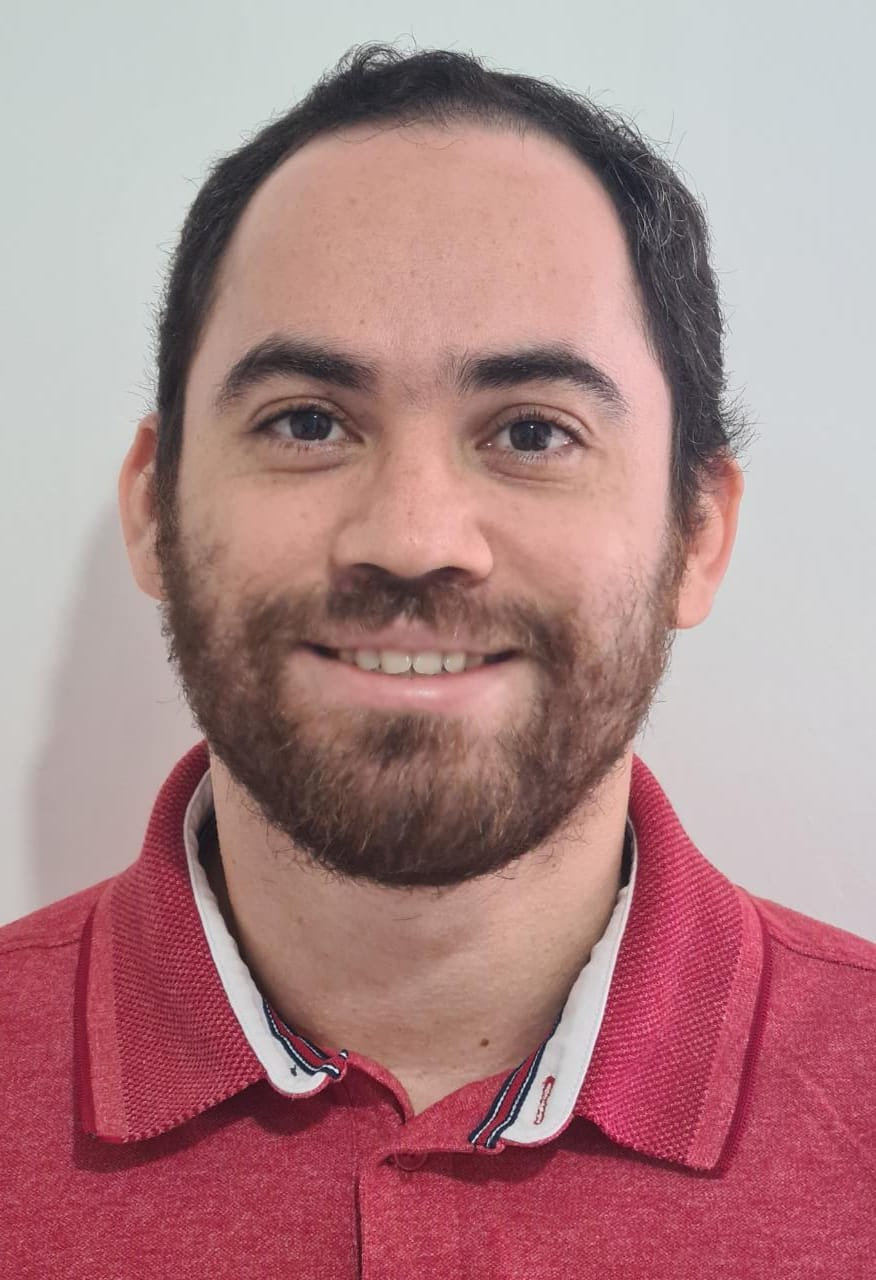
\includegraphics[scale=0.09]{imagens/fig-s20-plus-foto-lattes.jpeg}
 \end{flushright}

    \vspace{-9em}
    
    \begin{minipage}{.7\textwidth}
      \fontsize{10pt}{12}\selectfont{
    	\begin{itemize}%[<+->]  
    	    \item \autor, 39 anos (12/02)
    	    \item Sou técnico em Análise e Desenvolvimento de Sistema. Possuo Bacharelado nos cursos de Ciência da Computação (2011) e Sistemas de Informação (2016), participei do programa de Residência em Engenharia e Reuso de Software por meio da parceria da RiSE, Porto Digital e CPNq (2012). Tenho mestre e doutor em Ciência da Computação pelo CIn/UFPE. Atuo na indústria com desenvolvimento de software e na academia como professor.
        	\begin{itemize}%[<+->]  
        	    \item Java, Kafka, Postgresql, Docker, Angular, Spring...
        	    \item Análise e Desenvolvimento de Sistemas, Sistemas de Informação, Redes de Computadores.
        	\end{itemize}
    	\end{itemize}
    	}\par
    \end{minipage}

	\vspace{1em}
	\centering
\fontsize{20pt}{15.2}\selectfont{
    \url{http://www.brunomaciel.com}
	\vspace{1em}
	}\par
	
	
\end{frame}


\begin{frame}{Quem sou eu?}
% 	\begin{minipage}[r]{.15\textwidth}
% % 	\vspace{1cm}
%     \end{minipage}
%     \hfill\begin{flushright}% or better \raggedleft see comments below
%   \vspace{-3em}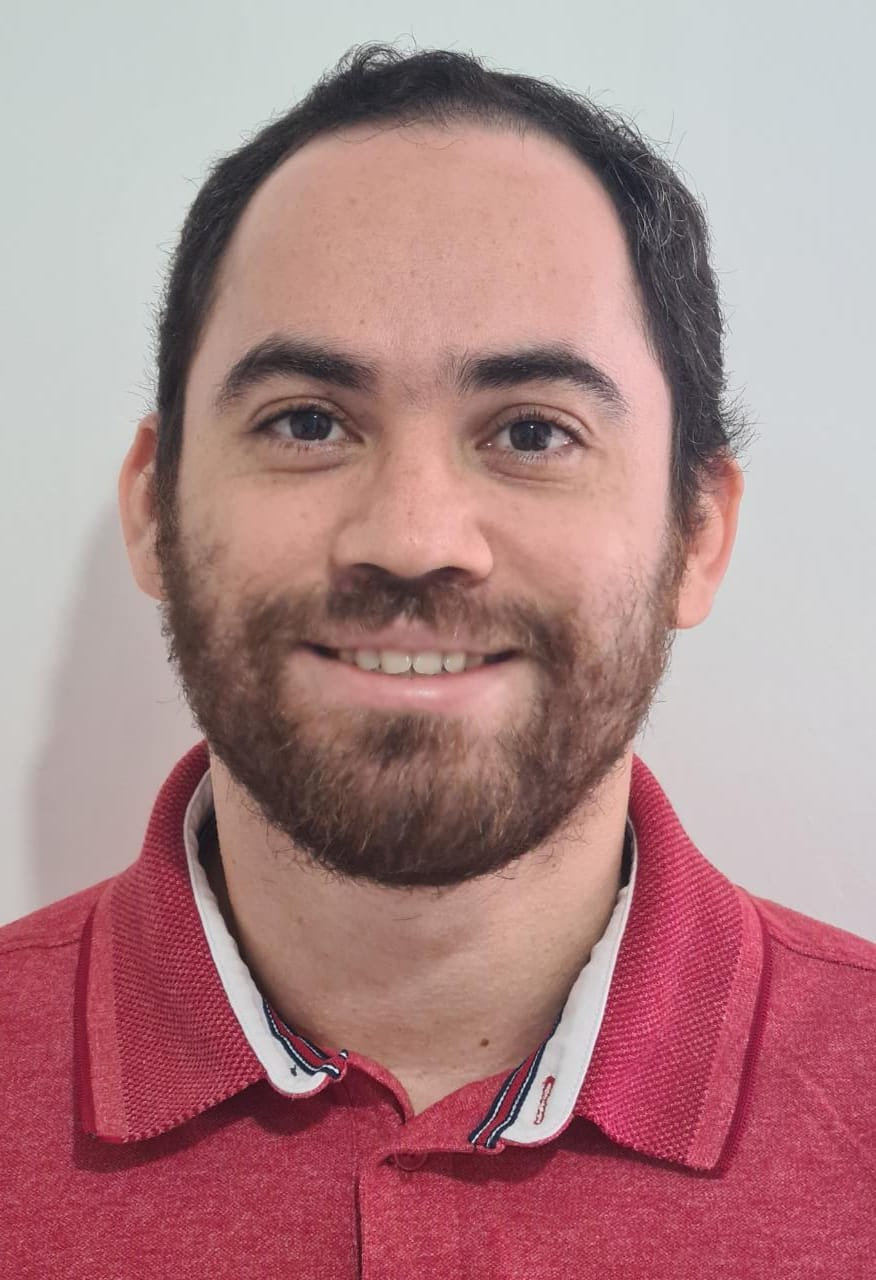
\includegraphics[scale=0.09]{imagens/fig-s20-plus-foto-lattes.jpeg}
%  \end{flushright}

%     \vspace{-10em}
    
    \begin{minipage}{.8\textwidth}
      \fontsize{10pt}{12}\selectfont{
    	\begin{itemize}%[<+->]  
    	   % \item \autor, 39 anos (12/02)
    	    \item Técnico em Análise e Desenvolvimento de Software, 2019-2020
    	    \item Doutor em Ciência da Computação, 2015-2020
    	    \item Mestre em Ciência da Computação, 2012-2014
    	    \item Especialista em Engenharia e Reúso de Software, 2011-2012
    	    \item Graduado em Sistemas de Informação, 2016-2016
    	    \item Graduado em Ciência da Computação, 2007-2011
    	    \item Técnico em Análise e Desenvolvimento de Software, 2007-2007
    	    \item CV completo \url{http://bit.ly/brunomaciel-lattes}
    	\end{itemize}
    	}\par
    \end{minipage}

	\vspace{1em}
	\centering
\fontsize{20pt}{15.2}\selectfont{
E-mail:	facir@brunomaciel.com
	\vspace{1em}
	}\par
	
\end{frame}


\begin{frame}{}
    \fontsize{14pt}{15.2}\selectfont{
	Apresentação pessoal, integração com a turma, introdução de conceitos básicos de banco de dados e despertar curiosidade alunos sobre o tema.
	
	\vspace{1em}
	}\par
	\vspace{1em}
\end{frame}


\begin{frame}{Aplicação de Avaliação}
    \fontsize{14pt}{15.2}\selectfont{
	Datas importantes
	\vspace{1em}
	}\par
	
	\fontsize{12pt}{15}\selectfont{
	\begin{itemize}%[<+->]  
	   % \item 30/09/2020 - Simulado da Primeira Avaliação (1A)
	    \item \textbf{01/04/2022 - Primeira Avaliação NP1}
	    \item 15/04/2022 - Feriado
	   % \item \textbf{18/11/2020 - Defesa dos projetos}
	   % \item 03/06/2020 - Simulado da Segunda Avaliação (2A)
	   % \item \textbf{01/04/2020 - Avaliação}
	    \item \textbf{20/05/2022 - Segunda Avaliação NP2} 
	    \item \textbf{03/06/2022 - Substitutiva}
	\end{itemize}
	
	}\par
	
	\vspace{1em}
\end{frame}



\begin{frame}{Compromisso semanal}
%     \fontsize{14pt}{15.2}\selectfont{
% 	Datas importantes
% 	\vspace{1em}
% 	}\par
	
	\fontsize{12pt}{15}\selectfont{
	\begin{itemize}%[<+->]  
	    \item Encontros: sextas
	    \item Período: %06/02/2020 à 04/06/2020
	    \item Início: 19h
	    \item Térmico: 21h50m
	   % \item Intervalo: 20h10m até 20h20m (a discutir)
	    \item Sala: 33
	\end{itemize}
	
	}\par
	
	\vspace{1em}
\end{frame}


\begin{frame}{Metodologia das Aulas}
Aulas:

    \fontsize{10pt}{12}\selectfont{
    \begin{itemize}%[<+->]  
        \item 19h-20h
        \item 20h-20h20m (intervalo)
        \item 20h20m-21h50m
	\end{itemize}
	}\par
	\vspace{0.5em}
	\fontsize{12pt}{15}\selectfont{
		\begin{itemize}%[<+->]  
	    \item Resolução de dúvidas gerais: 19h até 19h30m (30min)
	   % \item Revisão da aula passada: 19h20m até 19h40m (20min)
	   % \item Exercício em sala de aula: 19h40m até 19h50m (10min)
	    \item Adição de novos conteúdos: 19h30m até 21h50m
	   % \item Revisão/dúvidas do novo conteúdo: 21h20m até 21h30m (10m)
	\end{itemize}
	}\par
	\vspace{1em}
\end{frame}

\begin{frame}{Metodologia das Avaliação}

	\fontsize{12pt}{15}\selectfont{
	\begin{itemize}%[<+->]  
	    \item Primeira nota: %(exercício + prova)
	        \begin{itemize}%[<+->]  
%        	    \item Exercícios (peso +1)
        	    \item Prova escrita (peso 10)
        	\end{itemize}
    	\item Segunda nota: %(exercício + prova + projeto)
	        \begin{itemize}%[<+->]  
        	   % \item Exercícios (peso 1,5)        	    
        	   % \item Projeto (peso 1,5)
        	   % \item Participação - Frequência em aulas (peso 1)
        	    \item Prova escrita (peso 10)
        	\end{itemize}
	\end{itemize}
	}\par
	\vspace{1em}
\end{frame}

% \begin{frame}{Avisos}

% 	\fontsize{12pt}{15}\selectfont{
% 	\begin{itemize}%[<+->]  
% 	    \item Frequência escolar:
% 	        \begin{itemize}%[<+->]  
%         	    \item Número de faltas maior que 25\% = |Reprovado por faltas|
%         	    \item Cada dia de aula faltado equivale à 3 faltas;
%         	    \item Há 15 dias de aulas no cronograma |15 = 100\%|;
%         	    \item 4 dias faltados equivale a $\pm$ 26\%.
%          	\end{itemize}
%     	\item Atraso na entrega de atividade:
% 	        \begin{itemize}%[<+->]  
%         	    \item Cada dia atrasado tem penalidade de menos 10\% do peso.
%         	    \item Tempo máximo de atraso tolerado = 7 dias.
%         	\end{itemize}
% 	\end{itemize}
% 	}\par
% 	\vspace{1em}
% \end{frame}



\begin{frame}[t]{Ementa}
\vspace{1cm}
	\fontsize{12pt}{16}\selectfont{
	Conceituação de Organização e Arquitetura de Computadores e Máquinas Multiníveis. Organização de Sistemas Computacionais: CPU, Memória, Entradas e Multimídia e Barramentos. Nível Lógico Digital: Unidade Lógica e Aritmética, Organização de Memória, Clock e Registradores. Nível de Microarquitetura: Fluxos de Dados, Temporização do Fluxo de Dados, Operação de Memória, Microinstruções, O Mic-1, Exemplo de Macroarquitetura e Projeto do Nível de Microarquitetura (forma introdutória).
	}\par
	\vspace{1em}
\end{frame}

\begin{frame}[t]{Objetivos Gerais}
\vspace{1cm}
	\fontsize{12pt}{16}\selectfont{
	Entender o hardware de um sistema computacional. Entender o funcionamento dos vários módulos que compõem um sistema computacional.Conhecer a organização interna dos computadores, para análise da otimização do uso de seus componentes em aplicações das áreas de informação, comunicação e processos de controle.
	}\par
	\vspace{1em}
\end{frame}

\begin{frame}{Competências Específicas}

	\fontsize{12pt}{15}\selectfont{
% 	\begin{itemize}%[<+->]  
	   % \item 
	    Compreender a estrutura fundamental dos computadores e sua consequente organização, entendendo sua evolução, os conceitos fundamentais de seu próprio funcionamento e de seus componentes elementares, como processadores, memórias, sistemas de comunicação e dispositivos de entrada/saída.
% 	\end{itemize}
	}\par
	\vspace{1em}
\end{frame}



\begin{frame}{Avaliação}

	\fontsize{12pt}{15}\selectfont{
    Serão feitas avaliações, assim distribuídas:\vspace{1em}
	    
	\begin{itemize}%[<+->]  
	    \item Duas Notas do Professor (NP) para as atividades curriculares, com peso 4 (quatro) cada uma, na composição da nota semestral de cada disciplina;
	    
        \item Uma nota referente ao Projeto Integrado Multidiscipinar (PIM), com peso 2 (dois) no cálculo da Média Semestral (MS) de cada disciplina. Esse Projeto será desenvolvido durante o semestre.
        
        \item A MS será: (NP1 x 4 + PIM x 2 + NP2 x 4) / 10. Para a aprovação, a MS deverá ser igual ou superior a 5,0; é exigida a frequência mínima de 75\%. 
        
        \item O desempenho do aluno é avaliado numa escala de 0 (zero) a 10 (dez).
	\end{itemize}
	}\par
	\vspace{1em}
\end{frame}



\begin{frame}[t]{Bibliografia básica}
    \fontsize{12pt}{15.2}\selectfont{
	\vspace{1em}
	    \begin{itemize}
            \item DELGADO, José; RIBEIRO, Carlos. Arquitetura de Computadores. São Paulo: LTC, 2017.
            
            \item STALLINGS, W. Arquitetura e organização de computadores.10. ed. São Paulo: Prentice Hall, 2017.
            
            \item WIDMER, Neal S; TOCCI, Ronald J; MOSS, Gregory L. Sistemas Digitais. 12 ed. São Paulo: Pearson Education do Brasil, 2018.
            
            \item Mais informações é possível encontrar na ementa.
	    \end{itemize}
	}\par
\end{frame}


% \begin{frame}{Google sala de aula}
	
%     \hfill\begin{flushright}% or better \raggedleft see comments below
% 	 \vspace{-10mm}\includegraphics[width=25mm]{imagens/fig-qrcode-classroom.png}
% 	\end{flushright}


% %    \begin{wrapfigure}{r}{30mm}
% %    \vspace{-15mm}\qrcode[height=1in]{https://classroom.google.com}
% % 	\includegraphics[keepaspectratio=true,scale=0.4,trim=0cm 0 0 5cm]{imagens/qrcode.png}
% %	\end{wrapfigure}
% 	\vspace{-15mm}
	
%     \fontsize{14pt}{15.2}\selectfont{
% 	\vspace{1em}Código da turma \fontsize{34pt}{15.2}\selectfont{vigm76e}
% 	}\par
% 	\vspace{0.5em}

% 	\fontsize{10pt}{12}\selectfont{
% 	Vamos ter como recurso complementar o Google Sala de Aula [classroom]. Por lá vou deixar o material (slides, referências, atividades, etc.) que vocês vão utilizar durante o curso. Não preocupem-se, também vou deixar uma cópia do material (slides e atividades) disponível em pendrive e levarei comigo durante as aulas para os alunos que não puderem acessar o Google Classroom.
% 	\vspace{1em}
	
	
	
% 	Como usar o google sala de aula?

%     Use este tutorial \url{https://www.youtube.com/watch?v=l4oSdhLS5fQ} [vídeo] para te ajudar a entender o Google Classroom.

%     Clique na \url{https://classroom.google.com} para entrar no Google Classroom.

% 	}\par
% \end{frame}







% ----------------------------------------------------------
% ACRÔNIMO
% ----------------------------------------------------------
{\setbeamertemplate{footline}{} 
	\begin{frame}[allowframebreaks,noframenumbering,c]{Acrônimo}
		\vspace{2mm}
		\fontsize{11.2}{7.2}\selectfont{}
		\printglossary[type=\acronymtype,title=, toctitle=]
\end{frame}}




% ----------------------------------------------------------
% carrega os slides das aulas
% ----------------------------------------------------------

\ifnum \inputCurrentLesson=-1
    %importa automaticamente os arquivos de aulas
    \foreach\x in {1,...,\inputFilesMaxValue}{
        \IfFileExists{aulas/0\x.tex}{\input{aulas/0\x.tex}}{\IfFileExists{aulas/00\x.tex}{\input{aulas/00\x.tex}}{}}
    }
\else
    \ifnum \inputCurrentLesson>9 %`#\inputCurrentLesson>`9
        \input{aulas/0\inputCurrentLesson.tex}
    \else
        \input{aulas/00\inputCurrentLesson.tex}
    \fi
\fi





% ----------------------------------------------------------
% CAPA
% ----------------------------------------------------------
{\setbeamertemplate{footline}{} 
\setbeamertemplate{headline}{
\leavevmode%
  \hbox{%
    \begin{beamercolorbox}[wd=\paperwidth,ht=2.5ex,dp=1.125ex]{palette quaternary}%
    \end{beamercolorbox}%
  }
}
\begin{frame}[c,t]
	\maketitle
\end{frame}}





% ----------------------------------------------------------
% GLOSSÁRIO
% ----------------------------------------------------------
\begin{frame}[c,allowframebreaks,noframenumbering]{Glossário}
	\printglossary[title=, toctitle=]
\end{frame}


% ----------------------------------------------------------
% REFERÊNCIAS
% ----------------------------------------------------------
\part{Referências}
\frame{\partpage}
\nocite{*}
{
\setbeamertemplate{footline}{} 
\setbeamertemplate{headline}{
\leavevmode%
  \hbox{%
    \begin{beamercolorbox}[wd=\paperwidth,ht=2.5ex,dp=1.125ex]{palette quaternary}%
    \end{beamercolorbox}%
  }
}
\begin{frame}[allowframebreaks,noframenumbering]{Referências}
\fontsize{11.2}{7.2}\selectfont{}
\bibliographystyle{abbrvnat} %\usepackage{natbib}
\bibliography{referencias}
% \printbibliography
\end{frame}
}





% ----------------------------------------------------------
% incluir ementa dentro do material
% ----------------------------------------------------------
% \setbeamertemplate{background canvas}{}
% \include{plano-aulas}
% \includepdf[pages=-,fitpaper]{outros/ementa.pdf}
% % noautoscale
% % fitpaper
% %
% %
% %*******************************************************



\end{document}
